% Source: tex/chapters/ch06/09_ソフトウェアエンジニアリング運用ツール.tex
\subsubsection{監視とテレメトリ}

監視とテレメトリは、運用の中核である。監視は、サービスが正常かどうかを観察する活動である。テレメトリは、システムからデータを収集して分析に使う仕組みである。

監視では、アプリケーション層のログ、オペレーティングシステム層の実行トレース、サーバ層のCPU使用量やメモリ使用量などを収集する。収集されたデータには、統計分析や機械学習を使って意味を抽出できる。最終的には、ダッシュボードにより、開発者、運用者、製品責任者、経営層など、異なる利害関係者に必要な情報を見せる。

\begin{figure}[htbp]
\centering
\IfFileExists{assets/generated_figures/ch06/fig-ch06-12.png}{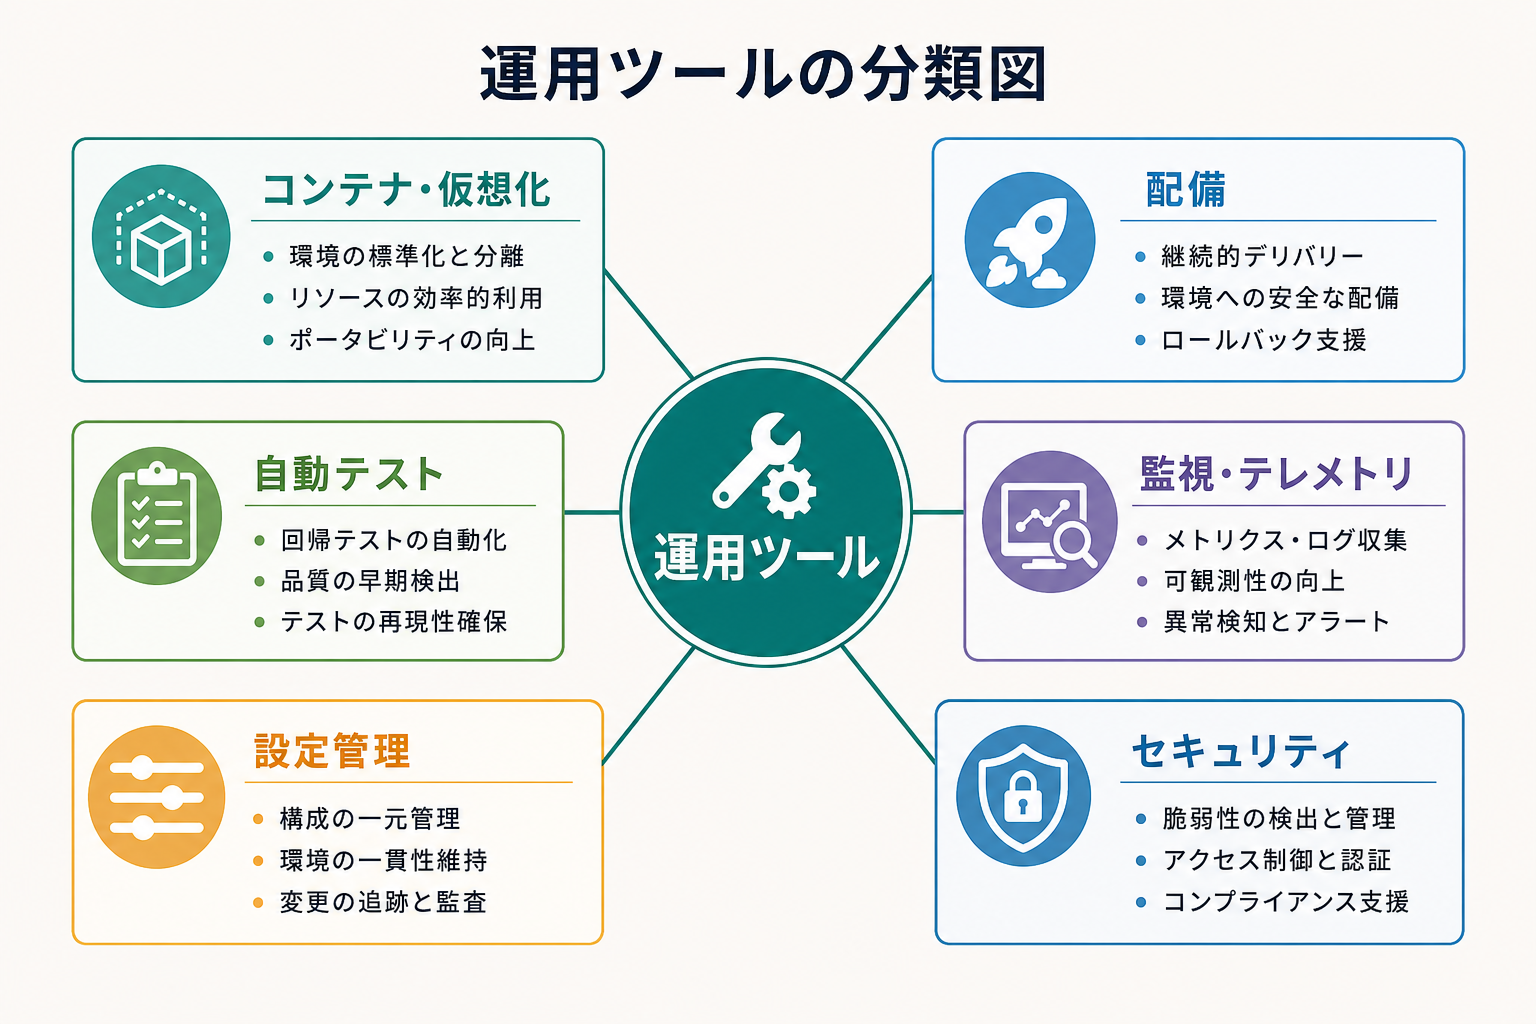
\includegraphics[width=0.96\linewidth]{assets/generated_figures/ch06/fig-ch06-12.png}}{\fbox{\parbox[c][48mm][c]{0.9\linewidth}{\centering 画像生成待ち\\運用ツールの分類図}}}
\caption{運用ツールの分類図}
\label{fig:ch06-12}
\end{figure}
